\documentclass[12pt]{article}

%% preamble: Keep it clean; only include those you need
\usepackage{amsmath}
\usepackage[margin = 1in]{geometry}
\usepackage{graphicx}
\usepackage{booktabs}
\usepackage{natbib}
\usepackage[T1]{fontenc}


% for space filling
\usepackage{lipsum}
% highlighting hyper links
\usepackage[colorlinks=true, citecolor=blue]{hyperref}


%% meta data

\title{Stats Paper Example}
\author{Okem Chime\\
  University of Connecticut
}

\begin{document}
\maketitle

\begin{abstract}
This is the abstract. The purpose of this part of the research paper is to
summarise the paper.
Beneath the neon sky, a symphony of unicorns pranced gracefully while juggling 
watermelons made of stardust. In the distance, a talking toaster serenaded a
curious platypus with a rendition of the national anthem of the moon. Suddenly,
a squadron of flying penguins wearing top hats descended from the clouds,
ushering in a parade of dancing teacups and sentient rubber chickens.
The entire scene was a kaleidoscope of surreal wonder, as if a fever dream
had collided with a whimsical fairy tale.
\end{abstract}


\section{Introduction}
\label{sec:intro}
The introduction is used to a refernce framework for the reader. 
The aim of this section is to answer three questions:
Why is the topic important/interesting?
What has been done on this topic in the literature?
What is your contribution?

The introduction section of a research paper serves as the gateway to the study,
playing a pivotal role in shaping the reader's understanding and engagement. 
Its importance lies in its ability to provide context, define the research
problem, and establish the rationale for the study. 

Here I am going to practice citing some works...

Some interesting research was done \citep{talovic2018strength} ...

...
\citet{oberstone2009differentiating} did something interesting research was done ...

% roadmap
The rest of the paper is organized as follows.
The data will be presented in Section~\ref{sec:data}.
The methods are described in Section~\ref{sec:meth}.
The results are reported in Section~\ref{sec:resu}.
A discussion concludes in Section~\ref{sec:disc}.


\section{Data}
\label{sec:data}

Utilize this segment to provide an account of the data essential for addressing
your research inquiries. Recall Pythagoras' theorem:
\begin{equation}
  \label{eq:pythag}
  a^2 + b^2 = c^2
\end{equation}
which states that the square of the adacent ($a^2$) of a triangle plus the square
of the opposte ($b^2$) equals the hypotensuse squared ($c^2$)

Equation ~ \eqref{eq:pythag} is useful for many applications ...

...


This is an inline equation: $ 180 / 3 = 60$ 
\section{Methods}
\label{sec:meth}


Utilize this section to introduce the methodologies that will produce results 
through the analysis of the provided data Suppose that the radius of a sphere 
is $r$. 
Then its area is:
\begin{equation}
  \label{eq:areaSphere}
  4\pi r^2.
\end{equation}

Equation~\eqref{eq:areaSphere} is interesting very useful... 



\section{Results}
\label{sec:resu}

Table~\ref{tab:rv} summarizes some data ...
\lipsum[1-4]

\begin{table}[tbp]
  \caption{This is my first table.}
  \label{tab:rv}
\centering
\begin{tabular}{rrr}
  \toprule
Left & Middle & Right \\ 
  \midrule
  A & B & C \\ 
  D & E & F \\ 
  H & I & J \\ 
  K & L & M \\ 
  N & O & P \\ 
  Q & R & S \\ 
  T & U & V \\ 
  W & X & Y \\ 
   \bottomrule
\end{tabular}
\end{table}

Figure~\ref{fig:myfig} shows ...


\begin{figure}[tbp]
  \centering
  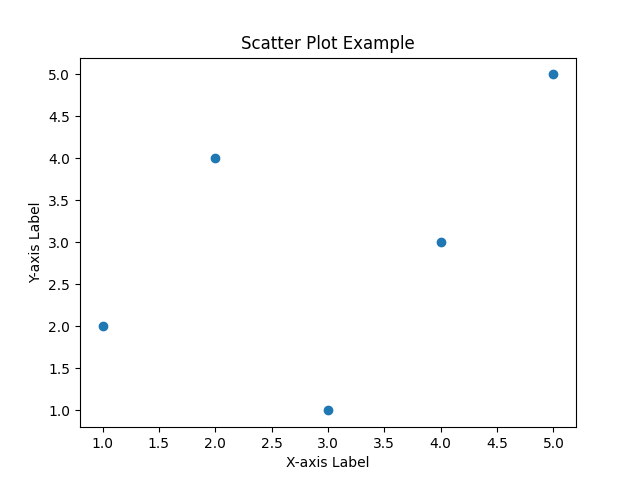
\includegraphics[width=\textwidth]{myfigure.png}
  \caption{This is my first figure.}
  \label{fig:myfig}
\end{figure}

\section{Discussion}
\label{sec:disc}

What are the main contributions again?

What are the limitations of this study?

What are worth pursuing further in the future?

\lipsum[1-2]


\bibliography{refs}
\bibliographystyle{plainnat} 


\end{document}